\subsection{Design}

\subsubsection{Stage 1}
At first stage, we have a look at what our goal is. To explain it from top perspective, we are looking to have a connection to API which is going to access database.
\newline
\begin{figure}[H]
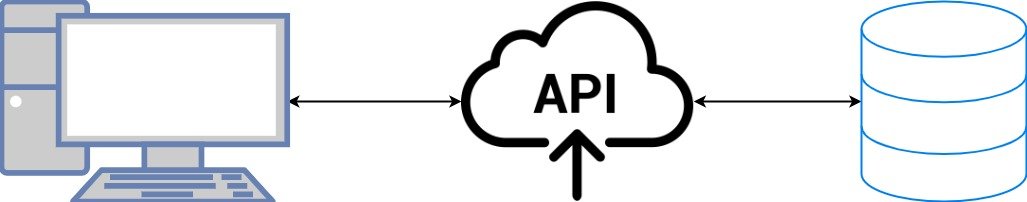
\includegraphics[scale=0.3]{img/systemDiagram-simplev.jpg}
\centering
\caption{Diagram of stage 1}
\end{figure}

\subsubsection{Stage 2}
In the second stage, we define our tools. For database, it is going to be MongoDB. API used for connections is Node with Express (and Mongoose) API. Then we serve the data to the users as NodeJS website or to IoT devices.
\newline
\begin{figure}[H]
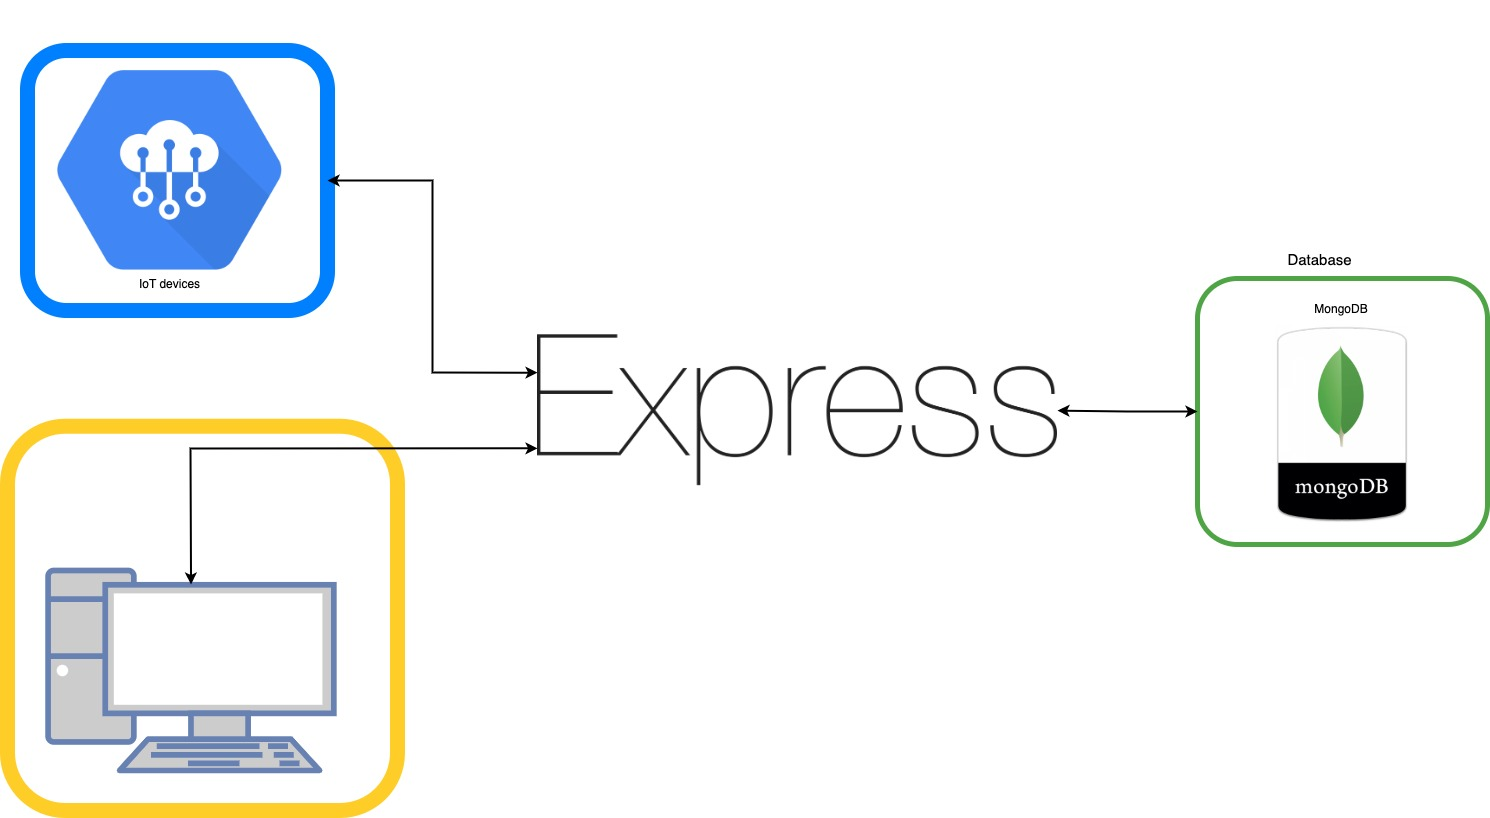
\includegraphics[scale=0.3]{img/systemDiagram-simplev2.jpg}
\centering
\caption{Diagram of stage 2}
\end{figure}

\subsubsection{Stage 3}
Third step defines structure for database and IoT. As seen in the diagram, Docker containers are going to be used for running the database. To improve database up time, we are going to shard it. 
This gives us 5 docker containers:
\begin{itemize}
  \item 1 primary node - all of the writes come to this node
  \item 2 secondary nodes - reads are done from secondary node to balance load off the main node. 
  \item 1 arbiter - in case that primary node goes down, this node is a tiebreaker of election between two of the nodes. This node cannot become primary node.
  \item 1 hidden node - this is backup node. It is hidden, meaning that it cannot participate in election process or in tie breaking. The only duty it has is to copy data from main node to itself. In case there is data loss, this node should have backups.
\end{itemize}
We have also expended on IoT side. Onece connection comes from API, it goes to user or IoT. Our API cannot communicate directly with IoT devices, but it needs some sort of "man in the middle". For that, we would expect API to communicate with the protocols (Apple home kit, Google home, Zigbee, Zwave) and they would comunicate with devices.
\newline
\begin{figure}[H]
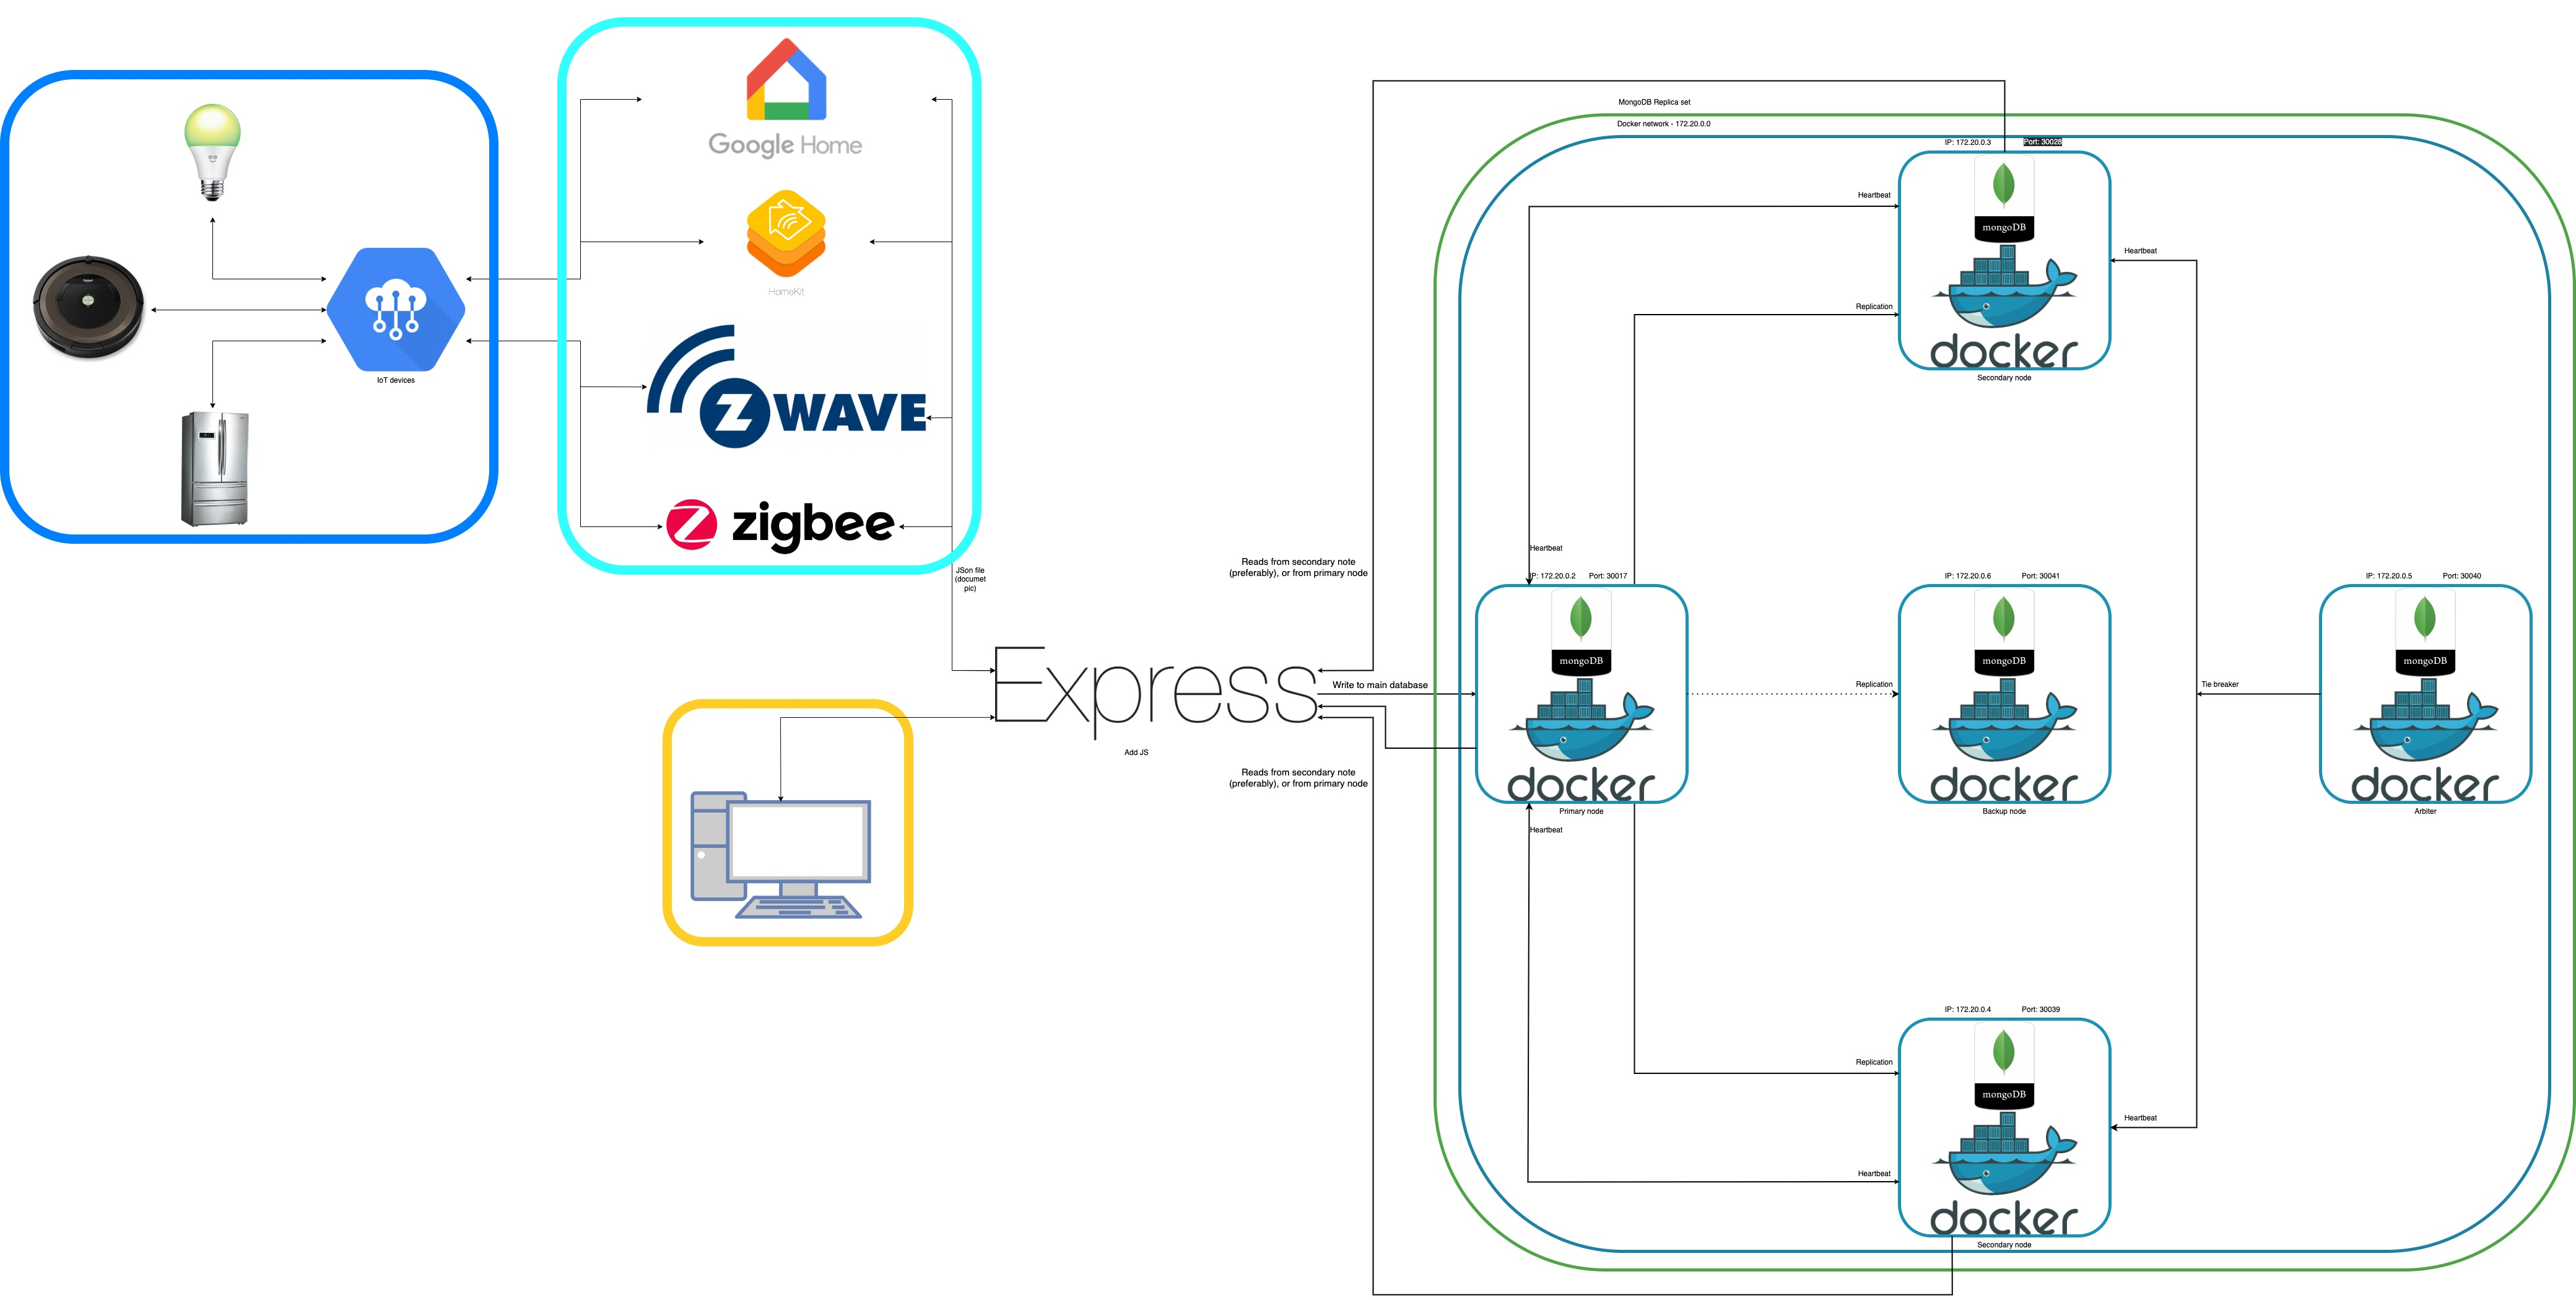
\includegraphics[scale=0.1]{img/systemDiagram-sharded.jpg}
\centering
\caption{Diagram of stage 3}
\end{figure}

\subsubsection{Stage 4}
In stage four, we upgrade our sharded database structure to clustered database structure. With that in mind, shard from step 3 was duplicated to create shard 1-3. With this, two shards can go "offline" and we would still have our data. As seen, we have added 3 new docker containers between API and our cluster. Those are routers. Router is "directing" the traffic between API and shards in our cluster. We have 3 routers in case one of them goes down.
\newline
\begin{figure}[H]
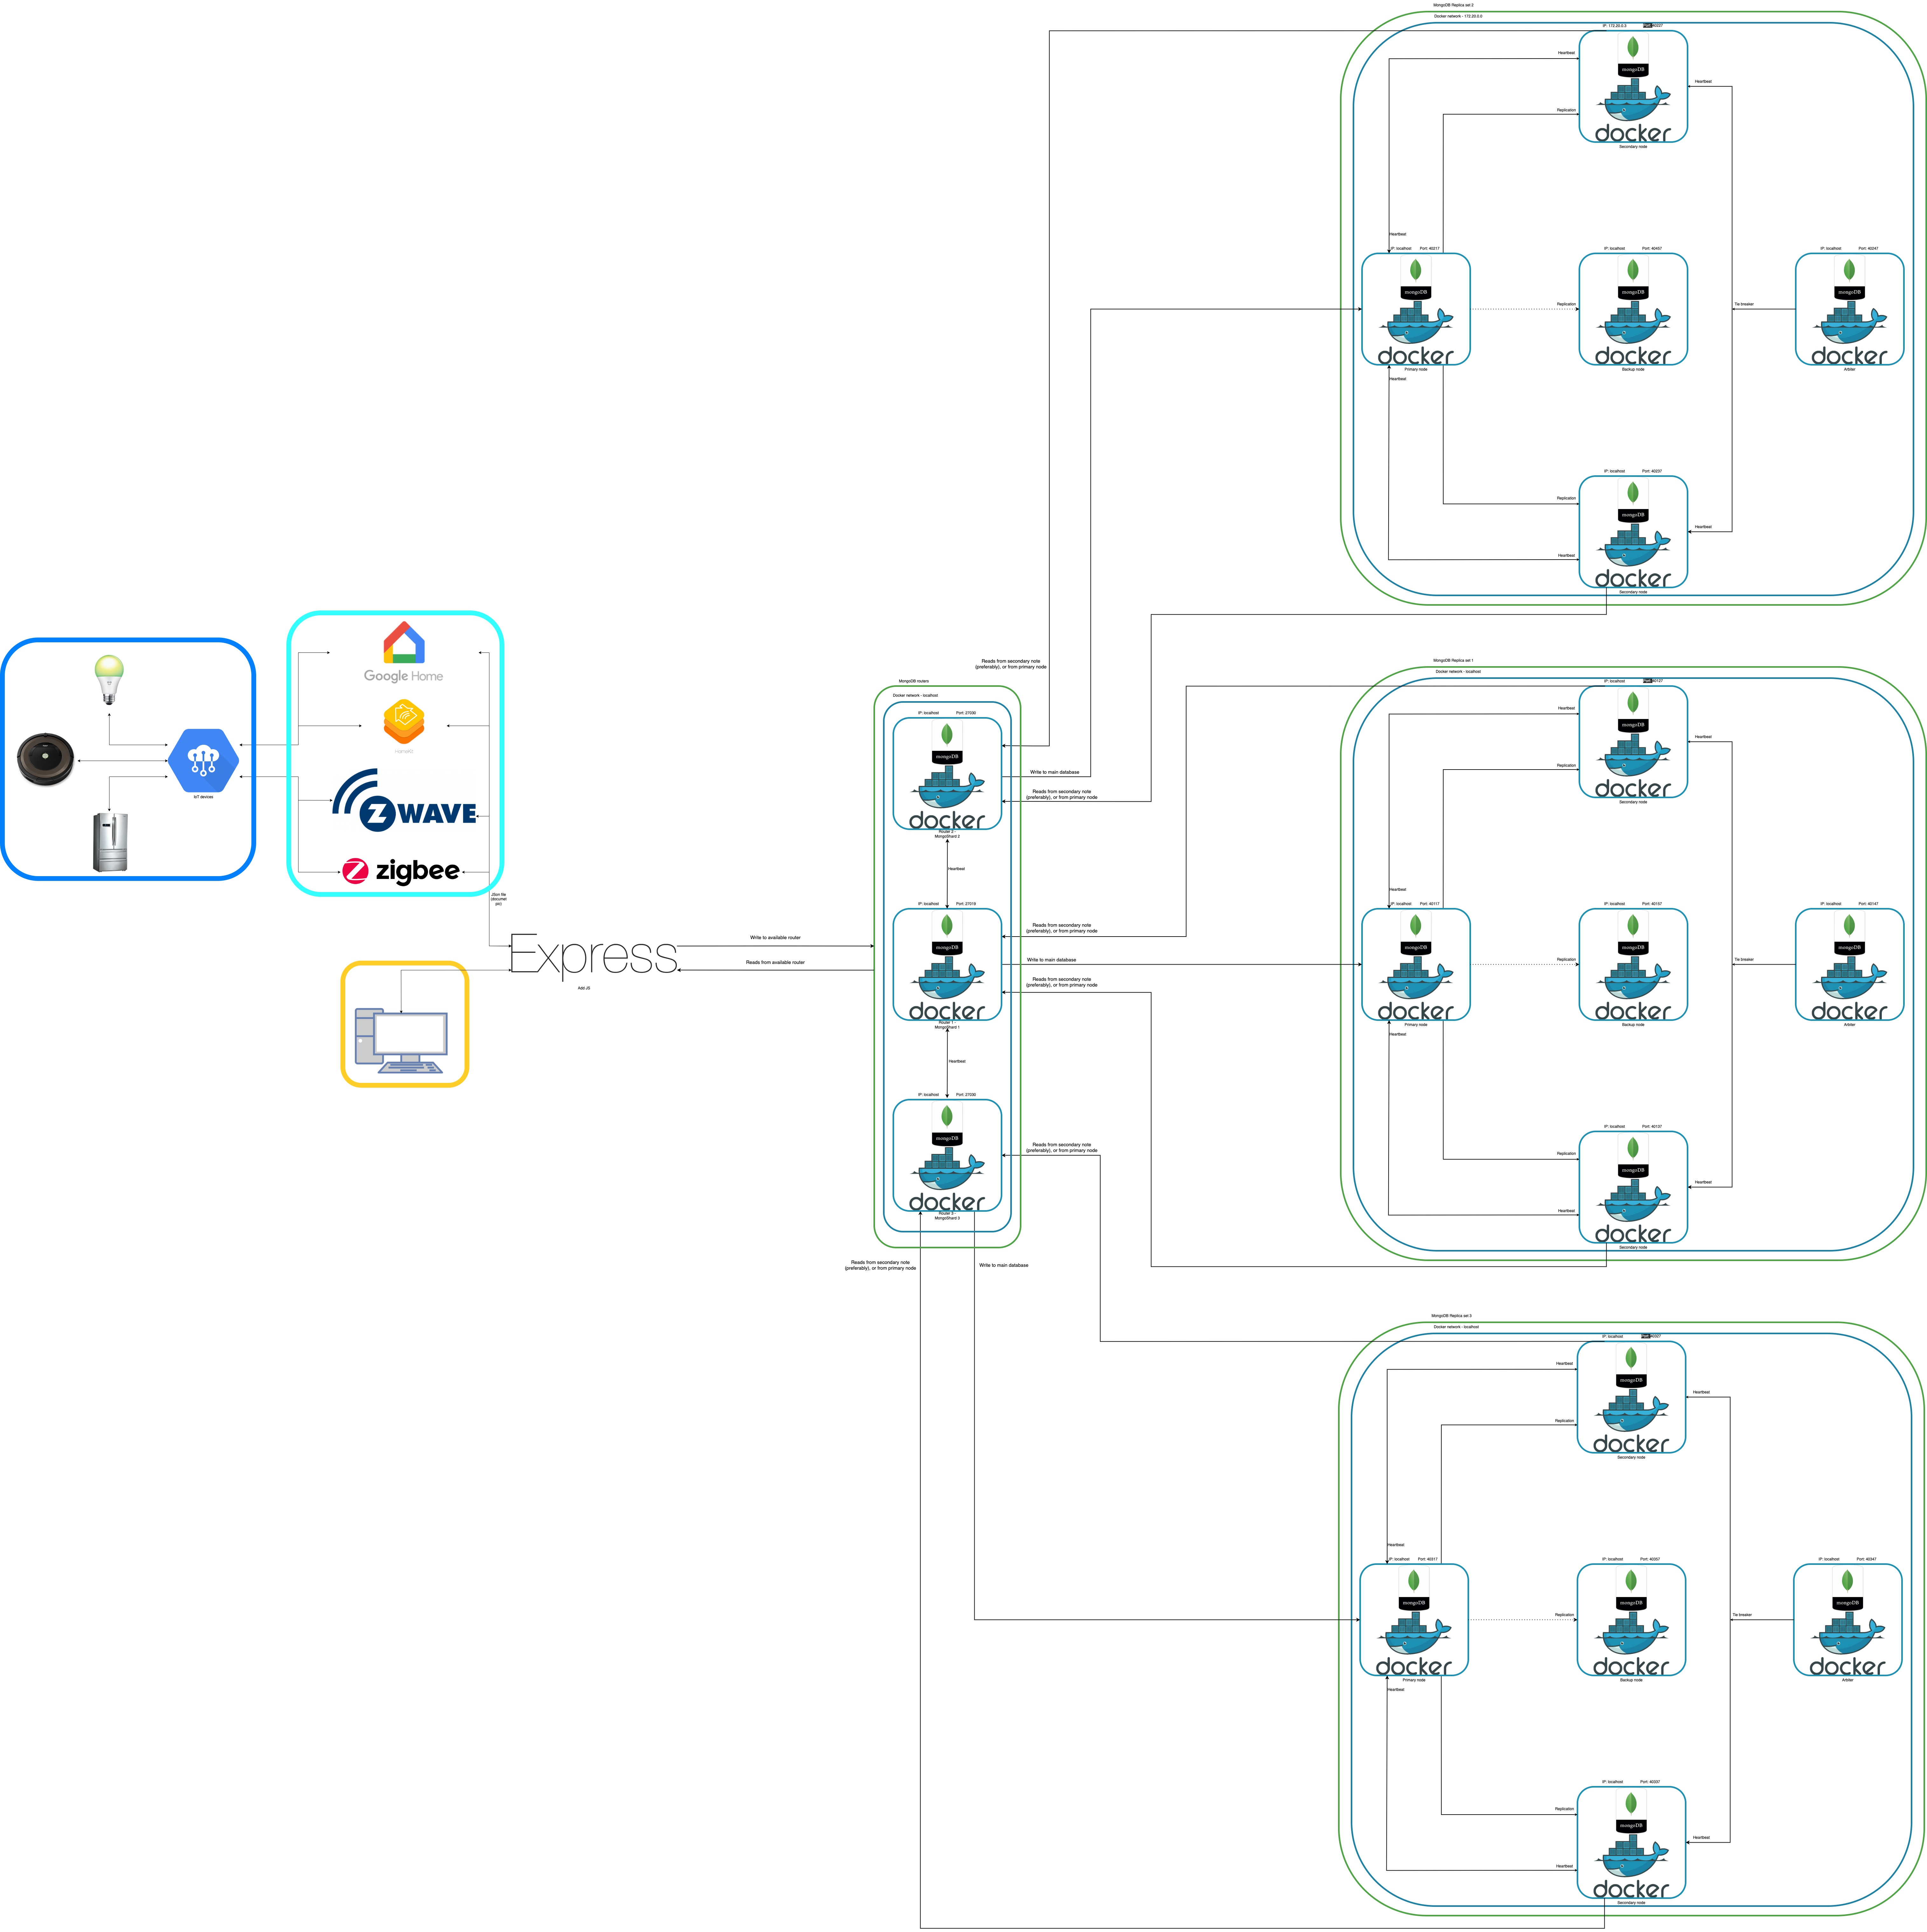
\includegraphics[scale=0.07]{img/systemDiagram-clustered.jpg}
\centering
\caption{Diagram of stage 4}
\end{figure}

\subsubsection{Stage 5}
The final stage is just a concept of security. If we wanted to have all of the connections secured behind the private network (for security reasons), we would put a VPN in front of API. With that, users with VPN credentials can connect to API. Since devices cannot connect directly to VPN (except if network would route directly to VPN), we would configure API to allow reads or writes from the protocols. With that, IoT devices can still communicate with our network but "hackers" cannot get to our API. If we wanted to add extra security, protocols would be set to read only outside of VPN.
\newline
\begin{figure}[H]
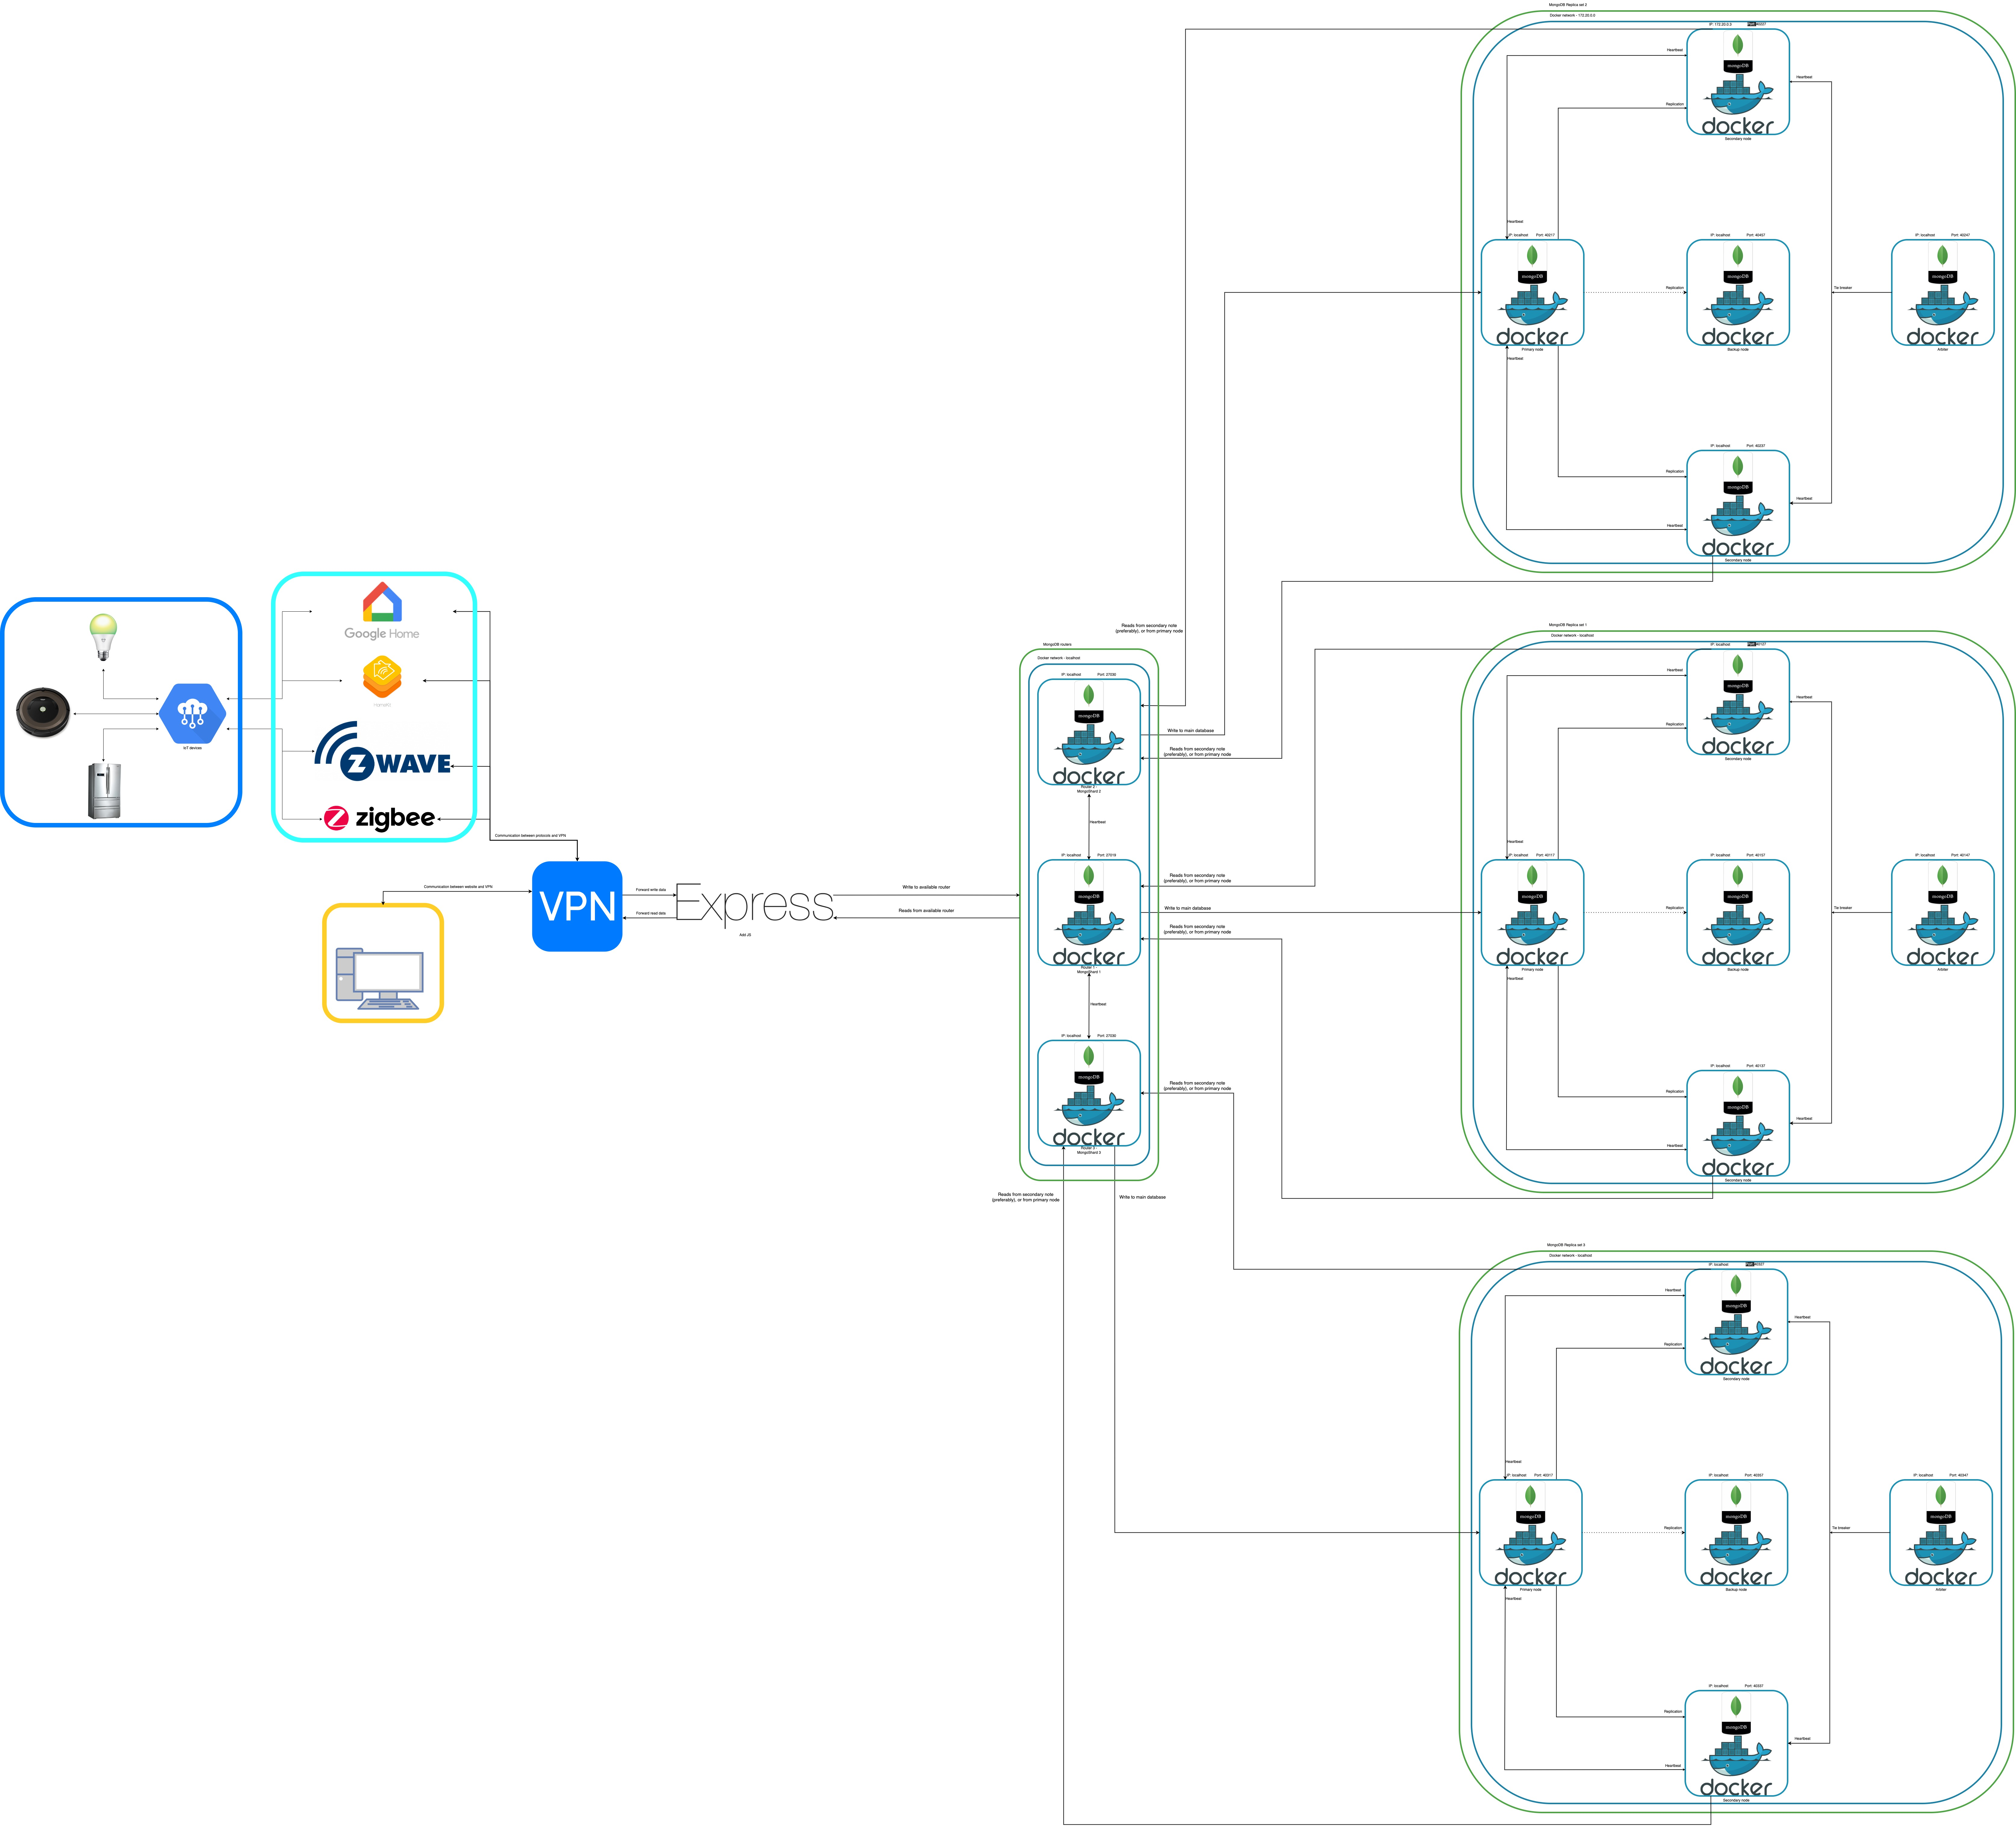
\includegraphics[scale=0.06]{img/systemDiagram-clusteredWithVPN.jpg}
\centering
\caption{Diagram of stage 5}
\end{figure}

As seen from the diagrams above, Docker \parencite{rad2017introduction} is going to be used for hosting the MongoDB \parencite{web:MongoDocker}. Reasons for that are: efficiently, simplicity and scalability.
\begin{center}
\begin{longtable}{ |m{4cm}|m{9cm}| } 
 \hline
 Reasoning & Description \\ 
 \hline
  Efficiently & 
  \begin{itemize}
    \item Docker containers are more light weight in comparison to VMs. This gives them an advantage in terms of OS storage and speed.
  \end{itemize} \\ 
  \hline
  Simplicity & 
  \begin{itemize}
    \item Starting up new docker container is simple. For our use case, we are using Docker Compose. With this, we can have predefined YAML file that has specifications for desired Docker container.
  \end{itemize} \\ 
   \hline
  Scalability & 
  \begin{itemize}
    \item Scaling with MongoDB and Docker is simple. We can scale vertically by adding more docker containers to our network or upgrading existing host server.
  \end{itemize} \\ 
 \hline
\caption{Reasons to use docker}
\end{longtable}
\end{center}


For our IoT database, we are using 4 collections:
\begin{center}
\begin{longtable}{ |m{4cm}|m{9cm}| } 
 \hline
 Collection name & Collection description \\ 
 \hline
  users & 
  \begin{itemize}
    \item has user data inside
    \item read writes from users and admins
  \end{itemize} \\ 
  \hline
  iot{\_}customer{\_}devices & 
  \begin{itemize}
    \item saves customers devices
    \item read writes from users and admins
  \end{itemize} \\ 
   \hline
  iot{\_}device{\_}history & 
  \begin{itemize}
    \item historical list of device status changes
    \item read writes from users and admins
    \item this can be a capped collection, saving changes for a month
  \end{itemize} \\ 
   \hline
  iot{\_}device{\_}info & 
  \begin{itemize}
    \item devices that are supported in the application
    \item users are set to read only, while admins can do read and write
  \end{itemize} \\ 
 \hline
\caption{Collections from DB and their descriptions}
\end{longtable}
\end{center}


\begin{figure}[H]
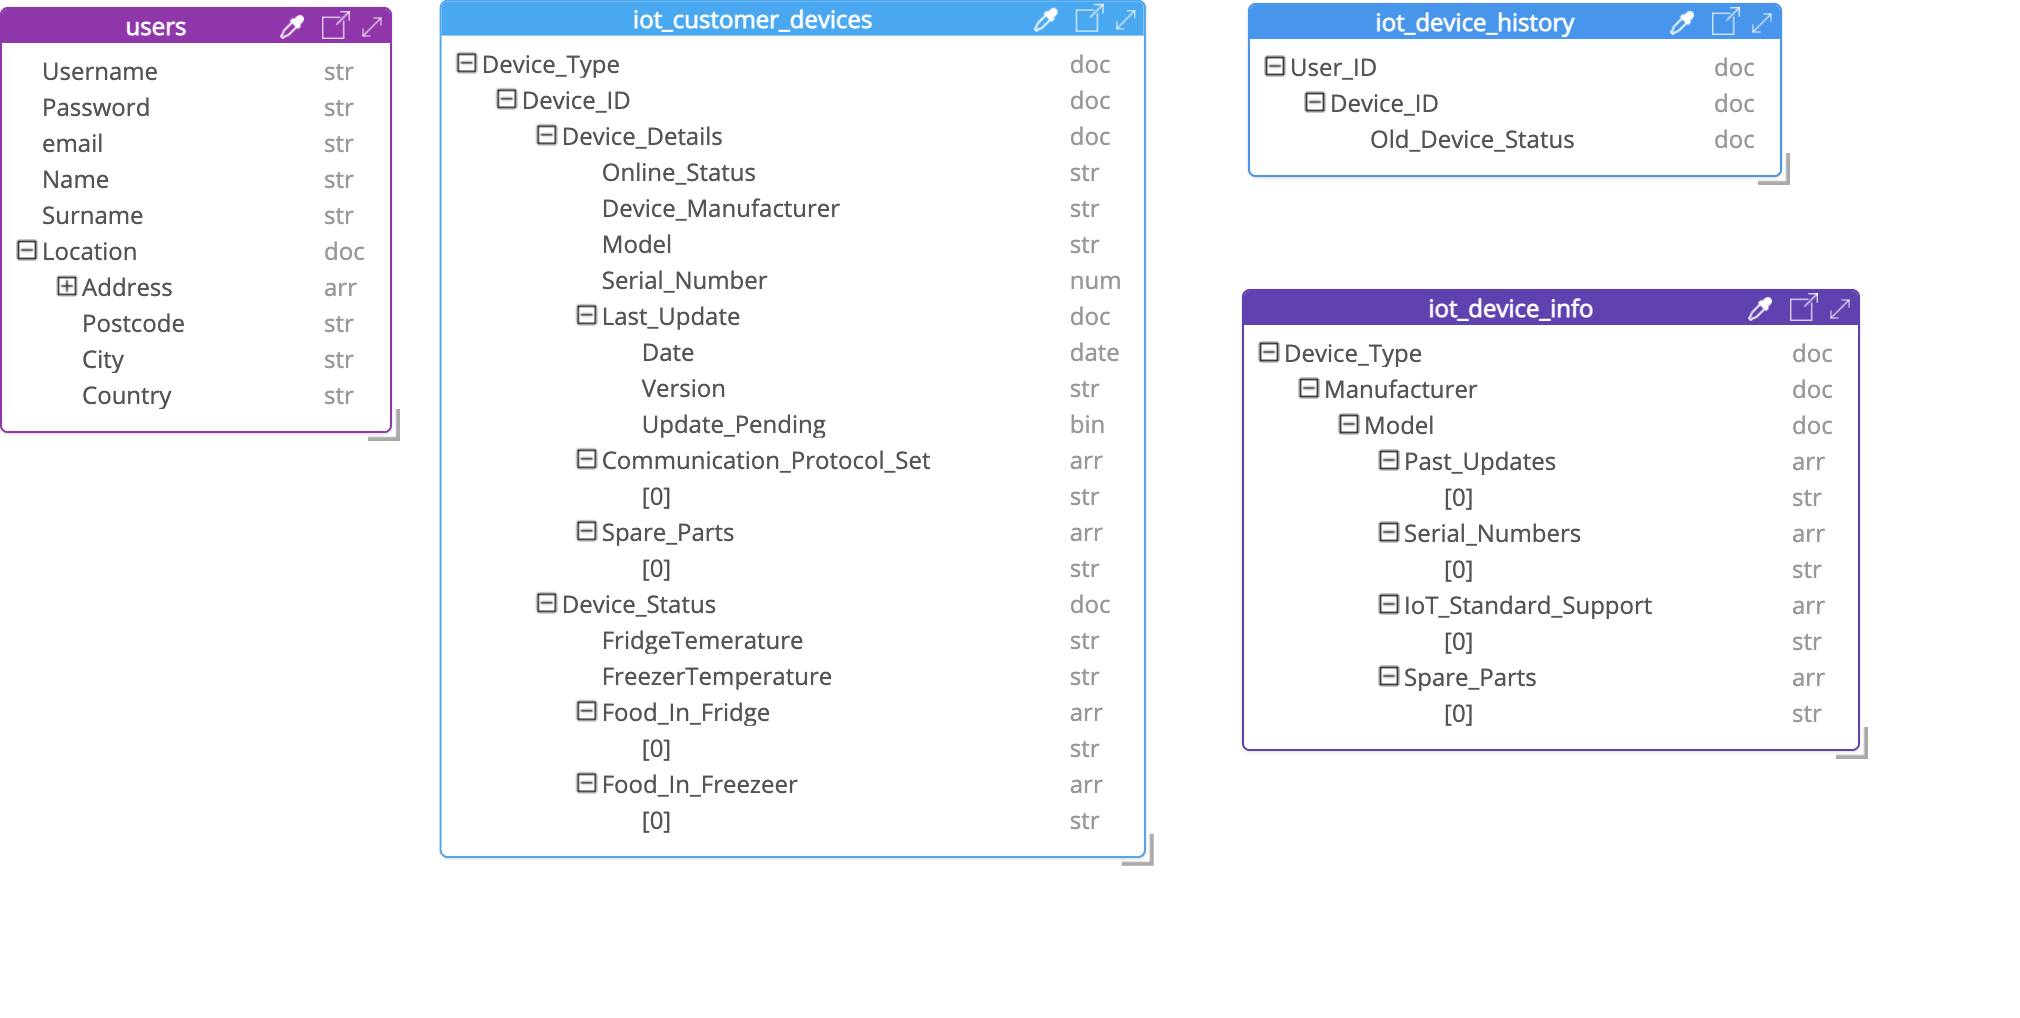
\includegraphics[scale=0.22]{img/IoT_Model_diagram.jpg}
\centering
\caption{Collections diagram}
\end{figure}

users collection document description:
\begin{center}
\begin{longtable}{ |m{4cm}|m{9cm}| } 
 \hline
  Document name & Document description \\ 
 \hline
  Username & 
  \begin{itemize}
    \item Type: string
    \item Must be unique username that would be at least 6 characters long.
  \end{itemize} \\ 
 \hline
  Password &   
  \begin{itemize}
    \item Type: string
    \item User defined password that is at least 8 characters long and it has symbols in. Cannot be the same as username or email.
  \end{itemize} \\
 \hline
  Email &   \begin{itemize}
    \item Type: string
    \item Must be unique and must meet certain expectations (example: have @ in string).
  \end{itemize} \\ 
 \hline
  Name &   \begin{itemize}
    \item Type: String
    \item Name of the user
  \end{itemize} \\
 \hline
  Surname &   
  \begin{itemize}
    \item Type: String
    \item Surname of the user
  \end{itemize} \\ 
 \hline
  Location &   
  \begin{itemize}
    \item Type: document
    \item Is build with 4 other sub items
        \begin{itemize}
            \item Address
                \begin{itemize}
                    \item Type: Array (length of 2)
                    \item Address line 1 is mandatory while address line 2 is optional
                \end{itemize}
            \item Postcode
                \begin{itemize}
                    \item Type: String
                    \item Postcode where user is located
                \end{itemize}
            \item City
                \begin{itemize}
                    \item Type: String
                    \item City where user is located
                \end{itemize}
            \item Country
                \begin{itemize}
                    \item Type: String
                    \item Country where user is located
                \end{itemize}
        \end{itemize}
 \end{itemize} \\
 \hline
\caption{Documents from users collection described}
\end{longtable}
\end{center}

iot{\_}customer{\_}devices collection document description
\begin{center}
\begin{longtable}{ |m{4cm}|m{9cm}| } 
 \hline
 Document name & Document description \\ 
 \hline
  Device{\_}Type &   
  \begin{itemize}
    \item Type: document
    \item Key is device name (example: smart{\_}light) and value is document which has devices inside
  \end{itemize} \\
 \hline
   Device{\_}ID &   
  \begin{itemize}
    \item Type: document
    \item Key is ID of device and value is device{\_}details and device{\_}status
  \end{itemize} \\
 \hline
   Device{\_}Details &   
  \begin{itemize}
    \item Type: document
    \item This document structure is the same across all the devices regardless of their type. Idea of this is to get device meta data which would be the same across the board.
    \begin{itemize}
        \item Online{\_}Status
        \begin{itemize}
            \item Type: boolian
            \item If the device is online or offline.
        \end{itemize}
        
        \item Device{\_}Manufacturer
        \begin{itemize}
            \item Type: String
            \item Who produced the device
        \end{itemize}
        
        \item Model
        \begin{itemize}
            \item Type: String
            \item Model name
        \end{itemize}
        
        \item Serial{\_}Number
        \begin{itemize}
            \item Type: number or String
            \item Serial{\_}number of the device.
        \end{itemize}
        
        \item Last{\_}Update
        \begin{itemize}
            \item Type: document
            \item When was device last updated.
        \end{itemize}
        
        \item Communication{\_}Protocol{\_}Set
        \begin{itemize}
            \item Type: array
            \item Based on available communication protocols, what protocols are being used.
        \end{itemize}
        
        \item Spare{\_}Parts
        \begin{itemize}
            \item Type: array
            \item If there are any spare parts available for purchase, they are listed here.
        \end{itemize}
    \end{itemize} 
  \end{itemize} \\
 \hline
   Device{\_}Status &   
  \begin{itemize}
    \item Type: document
    \item This document depends on device type. In the image above we have an example of what it would look like for smart fridge. But the idea is that device{\_}status gathers data that is from hardware level (example: battery level or last charge, etc...).
  \end{itemize} \\
 \hline
\caption{Documents from iot{\_}customer{\_}devices collection described}
\end{longtable}
\end{center}

iot{\_}device{\_}history collection document description
\begin{center}
\begin{longtable}{ |m{4cm}|m{9cm}| } 
 \hline
 Document name & Document description \\ 
 \hline
   User{\_}ID &  
  \begin{itemize}
    \item Type: document
    \item Key is User{\_}ID and value is document which has devices inside.
  \end{itemize} \\
  \hline
   Device{\_}ID &  
  \begin{itemize}
    \item Type: document
    \item Key is Device{\_}ID and value is old device status. When user updates device status, new version gets stored in the iot{\_}customer{\_}devices collection and old version gets written here.
  \end{itemize} \\
 \hline
\caption{Documents from iot{\_}device{\_}history collection described}
\end{longtable}
\end{center}

iot{\_}device{\_}info collection document description
\begin{center}
\begin{longtable}{ |m{4cm}|m{9cm}| } 
 \hline
 Document name & Document description \\ 
 \hline
  Device{\_}Type &   
  \begin{itemize}
    \item Type: document
    \item Key represents device name (example: Smart{\_}Vacuum). By theat, if we add new kind of device, we add new key (example: we don't have Smart{\_}TV so we create new key with that name). Value is manufacturers that produce that device.
  \end{itemize} \\
  \hline
  Manufacturer &  
  \begin{itemize}
    \item Type: document
    \item List of manufacturer names. Key is manufacturer name and value is model of device.
  \end{itemize} \\
  \hline
  Model &  
  \begin{itemize}
    \item Type: document
    \item Key represents model name and value represents information of the model
    \begin{itemize}
        \item Past{\_}Updates
        \begin{itemize}
            \item Type: array
            \item List of past updates.
        \end{itemize}
        
        \item Serial{\_}Numbers
        \begin{itemize}
            \item Type: array
            \item List of serial numbers that are registered on our platform under this model.
        \end{itemize}
        
        \item IoT{\_}Standard{\_}Support
        \begin{itemize}
            \item Type: array
            \item List of IoT standards that device supports.
        \end{itemize}
        
        \item Spare{\_}Parts
        \begin{itemize}
            \item Type: array
            \item List of spare parts that can be bought.
        \end{itemize}
    \end{itemize}
  \end{itemize} \\
  \hline
\caption{Documents from iot{\_}device{\_}info collection described}
\end{longtable}
\end{center}